\documentclass[11pt,]{article}
\usepackage[margin=1in]{geometry}
\newcommand*{\authorfont}{\fontfamily{phv}\selectfont}
\usepackage[]{mathpazo}

\usepackage{amssymb,amsmath}
\usepackage{xcolor}

%TIKZ and Flow chart material
\usepackage{tikz}
\usetikzlibrary{shapes.geometric, arrows}
\tikzstyle{startstop} = [rectangle, rounded corners, minimum width=3cm, minimum height=1cm,text centered, draw=black, fill=red!30]
\tikzstyle{io} = [trapezium, trapezium left angle=70, trapezium right angle=110, minimum width=3cm, minimum height=1cm, text centered, draw=black,fill=white]
\tikzstyle{process} = [rectangle, minimum width=3cm, minimum height=1cm, text centered, draw=black, fill=white]
\tikzstyle{decision} = [diamond, minimum width=3cm, minimum height=1cm, text centered, draw=black, fill=white]
\tikzstyle{smalldecision} = [diamond, minimum width=1cm, minimum height=1cm, text centered, draw=black, fill=white]
\tikzstyle{arrow} = [thick,->,>=stealth]
\tikzstyle{line} = [thick,-]
\tikzstyle{dot} = [circle,inner sep=0.5pt,draw=black, fill=black]


%\tikzstyle{startstop} = [rectangle, rounded corners, minimum width=3cm, minimum height=1cm,text centered, %draw=black, fill=red!30]
%\tikzstyle{io} = [trapezium, trapezium left angle=70, trapezium right angle=110, minimum width=3cm, %minimum height=1cm, text centered, draw=black,fill=white]
%\tikzstyle{process} = [rectangle, minimum width=3cm, minimum height=1cm, text centered, draw=black, %fill=white]
%\tikzstyle{decision} = [diamond, minimum width=3cm, minimum height=1cm, text centered, draw=black, %fill=green!30]
%\tikzstyle{arrow} = [thick,->,>=stealth]




\usepackage{abstract}
\renewcommand{\abstractname}{}    % clear the title
\renewcommand{\absnamepos}{empty} % originally center
\newcommand{\blankline}{\quad\pagebreak[2]}

\providecommand{\tightlist}{%
  \setlength{\itemsep}{0pt}\setlength{\parskip}{0pt}}
\usepackage{longtable,booktabs}

\usepackage{parskip}
\usepackage{titlesec}
\titlespacing\section{0pt}{12pt plus 4pt minus 2pt}{6pt plus 2pt minus 2pt}
\titlespacing\subsection{0pt}{12pt plus 4pt minus 2pt}{6pt plus 2pt minus 2pt}

\titleformat*{\subsubsection}{\normalsize\itshape}

\usepackage{titling}
\setlength{\droptitle}{-.25cm}

%\setlength{\parindent}{0pt}
%\setlength{\parskip}{6pt plus 2pt minus 1pt}
%\setlength{\emergencystretch}{3em}  % prevent overfull lines

\usepackage[T1]{fontenc}
\usepackage[utf8]{inputenc}

\usepackage{fancyhdr}
\pagestyle{fancy}
\usepackage{lastpage}
\renewcommand{\headrulewidth}{0.3pt}
\renewcommand{\footrulewidth}{0.0pt}
%\lhead{\footnotesize Problem Set \#5 }
\lhead{\footnotesize BUEC 311: Problem Set \#5, Consumer Preferences}
\rhead{\footnotesize \today}
\lfoot{\small \copyright }
\cfoot{}
\rfoot{\small \thepage/\pageref*{LastPage}}

\fancypagestyle{firststyle}
{
\renewcommand{\headrulewidth}{0pt}%
   \fancyhf{}
   \fancyfoot[C]{\thepage/\pageref*{LastPage}}
}

%\def\labelitemi{--}
%\usepackage{enumitem}
%\setitemize[0]{leftmargin=25pt}
%\setenumerate[0]{leftmargin=25pt}




\makeatletter
\@ifpackageloaded{hyperref}{}{%
\ifxetex
  \usepackage[setpagesize=false, % page size defined by xetex
              unicode=false, % unicode breaks when used with xetex
              xetex]{hyperref}
\else
  \usepackage[unicode=true]{hyperref}
\fi
}
\@ifpackageloaded{color}{
    \PassOptionsToPackage{usenames,dvipsnames}{color}
}{%
    \usepackage[usenames,dvipsnames]{color}
}
\makeatother
\hypersetup{breaklinks=true,
            bookmarks=true,
            pdfauthor={},
             pdfkeywords = {},
            pdftitle={Problem Set \#5: Consumer Preferences},
            colorlinks=true,
            citecolor=blue,
            urlcolor=blue,
            linkcolor=magenta,
            pdfborder={0 0 0}}
\urlstyle{same}  % don't use monospace font for urls


\setcounter{secnumdepth}{0}


%



\usepackage{setspace}

\title{\vspace{-1.5cm}\Large{BUEC 311: Business Economics, Organization
and Management}\medskip\\\Large{Problem Set \#5}
\medskip\\\Large{Consumer Preferences}
}
\date{\vspace{-.75cm}\Large{\today}}

\definecolor{light-gray}{gray}{0.8}


\begin{document}

\vspace{-5cm}\maketitle
 \tikz [remember picture,overlay]
    %\node[yshift=-1.65cm,xshift=0cm] at (current page.north)
    %\node[yshift=-1.65cm,xshift=0cm] at (current page.north)
        %or: (current page.center)
        \node[yshift=-1cm,xshift=6.5cm] at (current page.north west)
        %{
\includegraphics[width=3in]{UA-ASB-COLOUR.png}};
        {
\includegraphics[width=.5\paperwidth]{../images/UA-ASB-COLOUR.png}};
\vspace{-.75cm}		
		\thispagestyle{firststyle}



\begin{enumerate}
\def\labelenumi{\arabic{enumi}.}
\tightlist
\item
  Suppose that Jim is contemplating whether to spend the money to buy a
  promotional ski card for this upcoming season. His utility function
  for skiing and all other goods is given by U=x*s+x, such that his
  marginal utility for skiing is given by \(U_s=x\) and his marginal
  utility for other consumption is \(U_x=s+1\). Assume that he has \$300
  of disposable income to allocate across these goods, and that the
  price of a daily lift ticket is \$100. Use a price of \$1 for the
  indexed other goods (i.e.~the budget constraint has intercept at x=300
  and s=3.)
\end{enumerate}

\begin{enumerate}
\def\labelenumi{\alph{enumi})}
\item
  With no promotional discount, and assuming he can only ski full days,
  how many days should Jim ski this year?
\item
  Now assume that a promotional card costs \$50 but offers half price
  lift tickets? Should Jim buy the card?
\item
  How many days will he ski once he has purchased the card?
\end{enumerate}

\newpage

\begin{enumerate}
\def\labelenumi{\arabic{enumi}.}
\setcounter{enumi}{1}
\tightlist
\item
  Janine is considering buying a Costco membership. If she buys the
  Costco membership, it will mean giving up one night out per month with
  her friends, but she'll have a lower cost of groceries. Assuming that
  she's currently spending 2 nights out per month with her friends and
  buying 2 carts of groceries per month, and that her preferences and
  budget constraint are shown on the map below, do you think she should
  buy the Costco membership if it reduces her cost of groceries by 50\%?
\end{enumerate}

\begin{center}
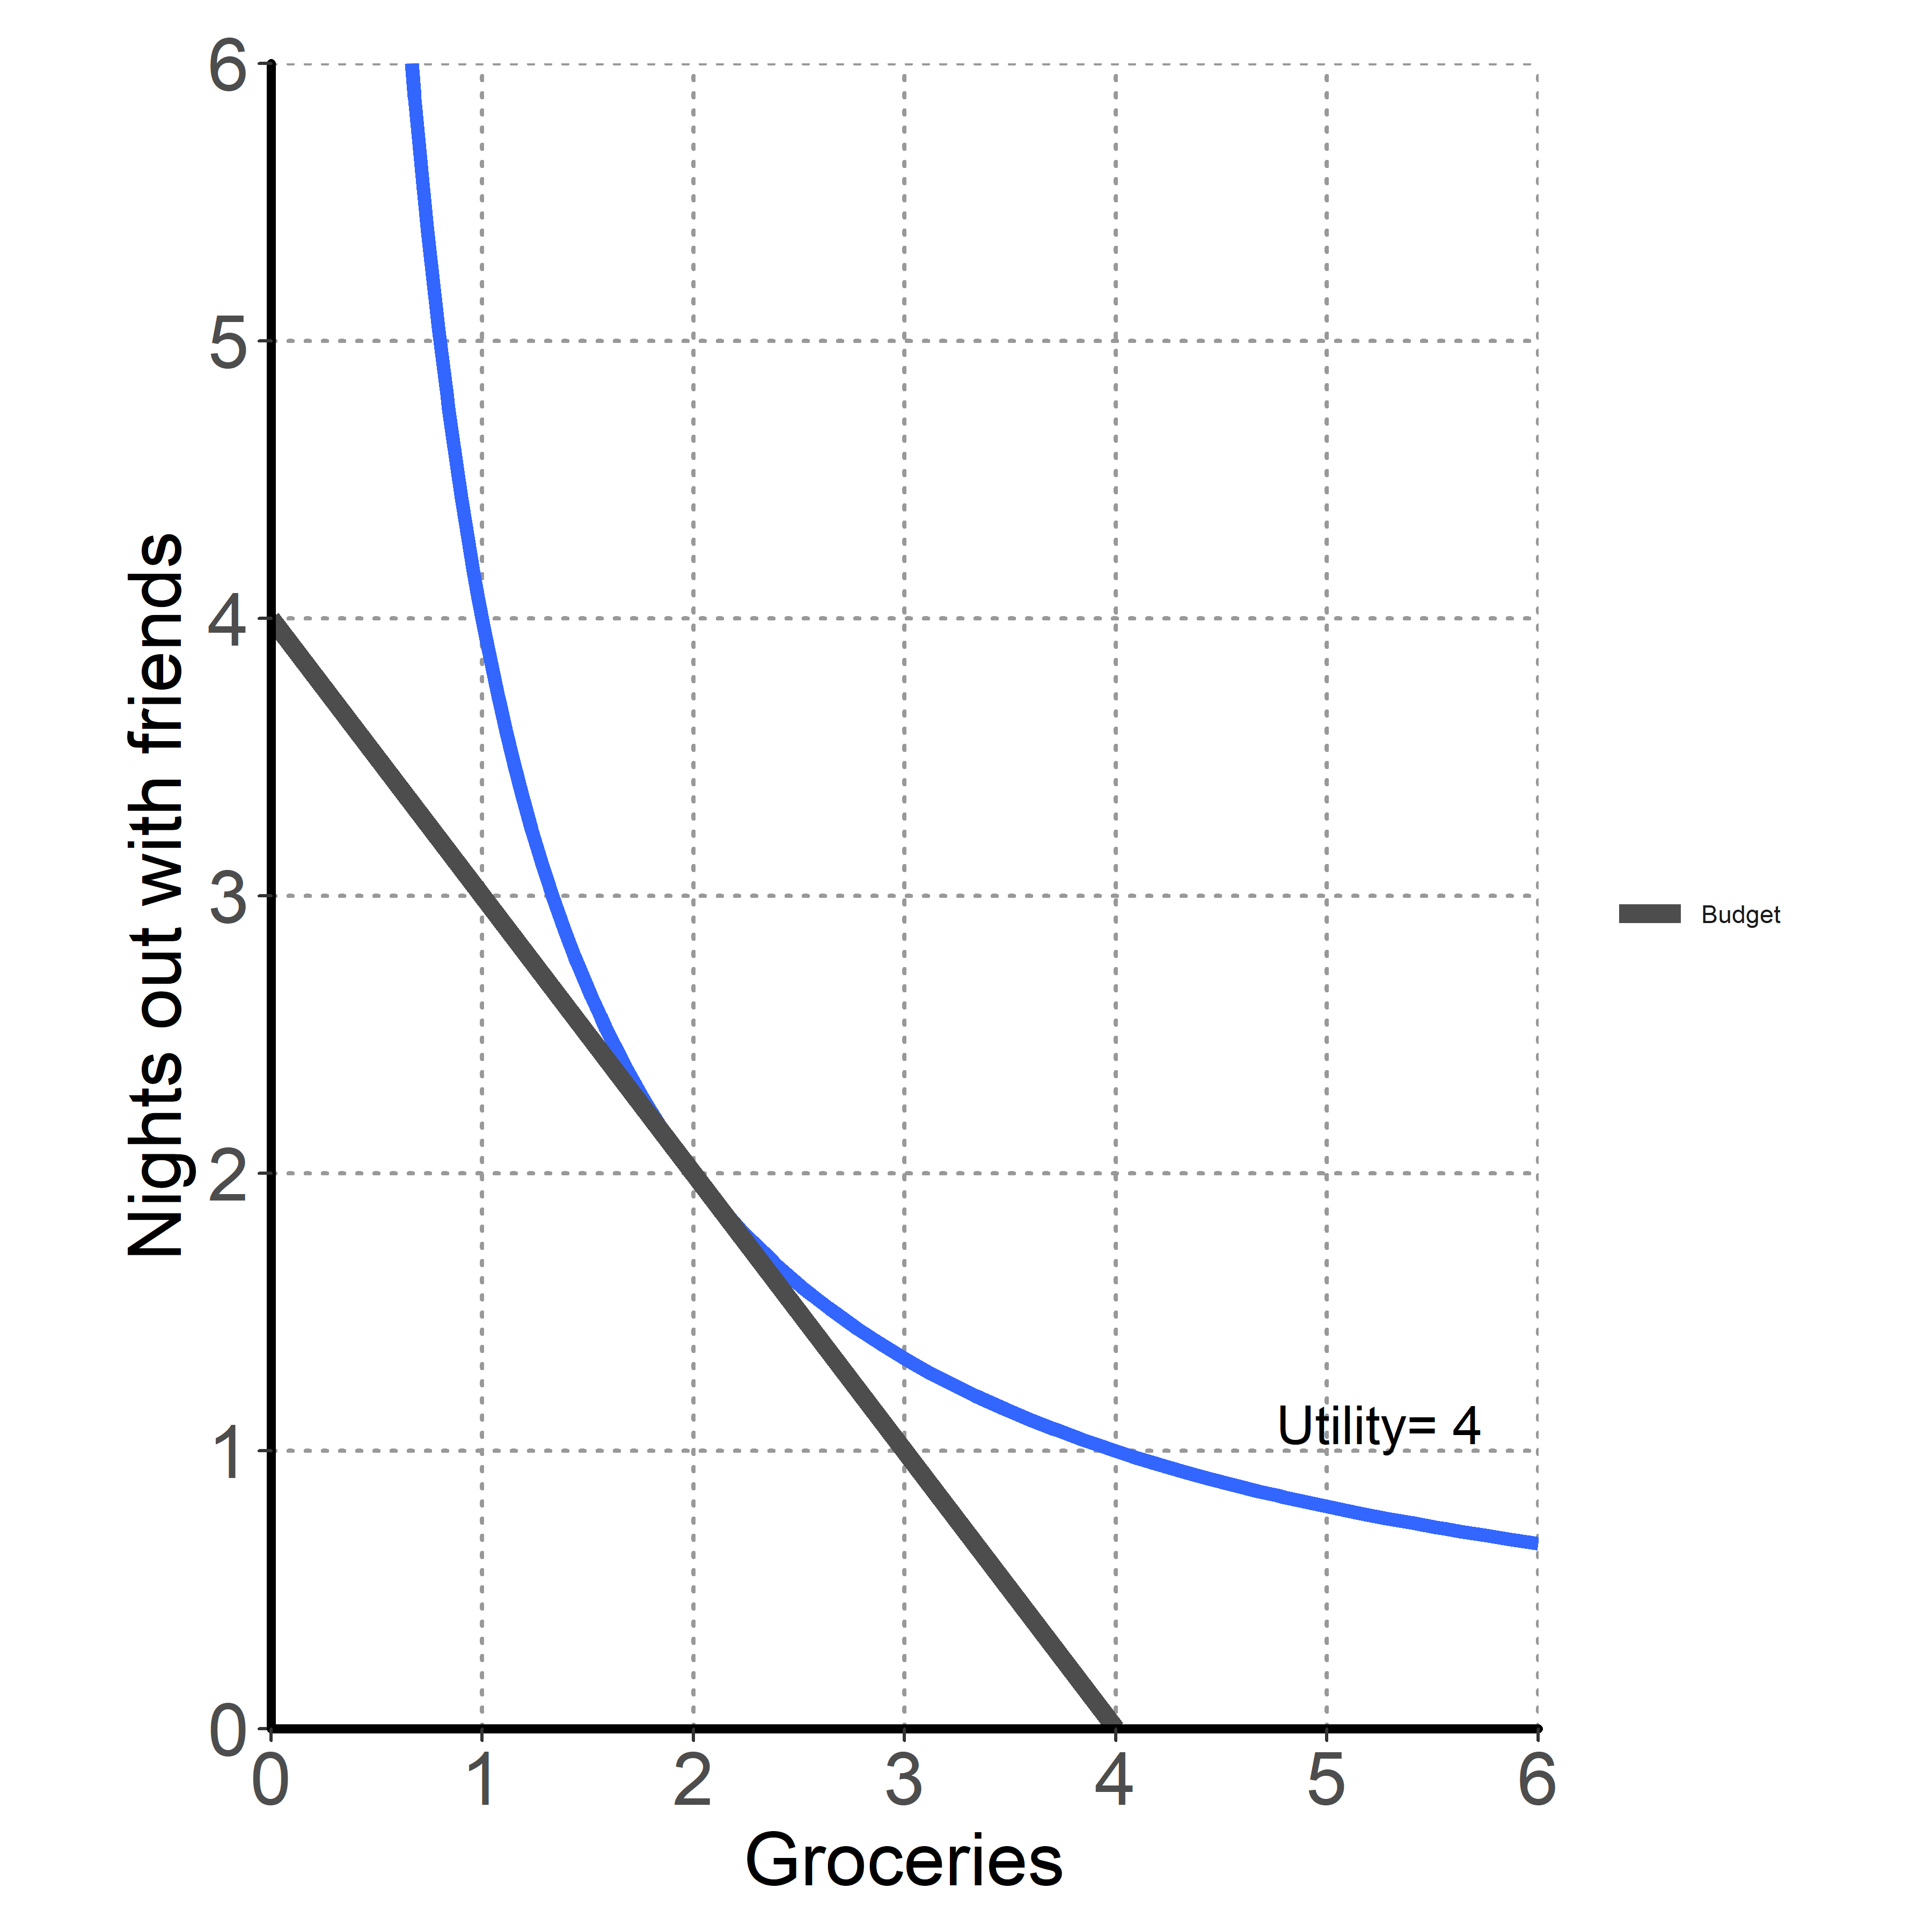
\includegraphics[width=0.65\textwidth]{../images/utils_costco.png}
\end{center}




\end{document}
